\chapter{SwiftのおよびC++の特徴と差異}
\label{differential}

本研究ではSelf-host化によってSwiftコンパイラの可読性を向上させることを目的としているが、その考えはSwiftで記述したSwiftコンパイラと現行のC++で記述されたコンパイラとで可読性に差が出るという仮説に基づいている。
本章では、その仮説が確からしいと考えている根拠となる各言語の差異について、それらの特徴を比較して説明する。

\section{比較する特徴}

本章ではSwiftとC++について以下3つの視点から特徴を述べる。

\begin{enumerate}
\item 言語パラダイム
\item 型システム
\item 制御構文
\end{enumerate}

まず、プログラミング言語が採用するプログラミングパラダイムはその言語に必要となる機能を決定し、たとえ新しい言語であったとしてもその構文はそれら機能の慣習的な表記法の影響を受ける
% 要出典
。そのため、プログラミングパラダイムはその言語の可読性を左右する一つの大きな要因となっており、本章で取り上げるべき特徴であるといえる。

次に、SwiftやC++のような静的型付言語では採用する型システムによってプログラムに対する意味付けの柔軟性が大きく左右される
% 要出典
。
うまく意味付けのできないプログラムは可読性を低下させうるため
% 要出典
、型システムについても本章で取り上げることとする。

最後に、分岐やループを作る制御構文はプログラムの流れを決定する役割を担うため、プログラムの流れの把握し易さにその設計が大きな影響を及ぼす
% 要出典
。
プログラムの流れを把握することがコードを読む大方の目的であるため、これも可読性に影響を与える1つの要因として本章で取り上げる。


\section{Swiftの特徴}
\label{differential:swift-features}

\subsection{言語パラダイム}

Swiftは近年の汎用言語に採用されている多くのプログラミングパラダイムを取り入れているマルチパラダイムプログラミング言語であり、以下のようなプログラミングパラダイムを採用している。

\subsubsection{関数型プログラミング}

Swiftでは関数を第一級のオブジェクトとして扱い、2つの型から成る関数型を用意することで、MLやHaskellなどの言語と同様のラムダ計算に近しい表記方法を行う関数型プログラミングが可能となっている。

Swiftにおける関数型プログラミングの例をプログラム~\ref{code:functional}に挙げる。
関数用の型が矢印演算子によって提供されており、関数自体を変数に代入して使用できていることがわかるだろう。

\begin{lstlisting}[caption=Swiftにおける関数型プログラミングの例, label=code:functional]
let f: Int -> Int = { x in x + 1 }
print(f(1)) // 標準出力に 2 と表示する
\end{lstlisting}

このパラダイムにより、関数を引数として受け取る高階関数を用いるなどして関数をより抽象化し、ボイラープレートを防ぐことができるようになる。
また、一般に関数の型はその表記が複雑化しやすいという問題があるが、Swiftでは型推論や型の別名定義などの手法によってこれを簡単に記述できるようになっている。

\subsubsection{オブジェクト指向プログラミング}

Swiftが提供する複合型であるクラス、構造体、列挙体、プロトコルでは継承関係を定義することができ、外部の手続きから呼び出し可能な値や他の型定義などのメンバを持つことができるように設計されていることで、オブジェクト指向プログラミングを可能としている。

Swiftにおけるオブジェクト指向プログラミングの例をプログラム~\ref{code:objective}に挙げる。
この例では継承関係のあるクラスから生成されたオブジェクトに対し、クラスで定義された関数のメンバを呼び出している。

\begin{lstlisting}[caption=Swiftにおけるオブジェクト指向プログラミングの例, label=code:objective]
class Parent {
    func f() { print("parent") }
}

class Child : Parent {
    override func f() { print("child") }
}

let x: Parent = Child()
x.f() // 標準出力に child と表示する
\end{lstlisting}

継承関係を持つことができる複合型はプログラムのカプセル化の礎を築きプログラムの再利用を容易にする他、関数や変数をメンバとして保持することでそれらの関係性をより明確に定義できるようになる。

\subsubsection{パターンマッチ}

Swiftは特定の構造を持つ値についてその一般的なパターンを定義し、変数を含む左辺値と変数を含まない右辺値を比較することで左辺値中の変数の型と値を決定するパターンマッチの機構を持っている。

Swiftにおけるパターンマッチの例をプログラム~\ref{code:pattern-match}に挙げる。
現在のSwiftではこの例内の6行目のような列挙体やタプルの値について特に柔軟なパターンマッチを提供している。

\begin{lstlisting}[caption=Swiftにおけるパターンマッチの例, label=code:pattern-match]
enum Sample {
    case X, Y(Int)
}
let x = Sample.Y(1)

if case Sample.Y(let v) = x {
    print(v) // 標準出力に 1 と表示する
}
\end{lstlisting}

パターンマッチでは値の構造を元にした処理の分岐を端的に記述することができ、パターンマッチ中の変数束縛や変数定義式でのパターンマッチは複数の値を同時に扱う自然な方法を提供する。


\subsection{型システム}

Swiftの型システムはその柔軟性によってプログラマの様々な意味を表現できるだけでなく、型推論によって煩雑な型の省略を可能にし、プログラムの可読性を向上している。
以下ではSwiftで採用されている型システムの特徴について述べる。

\subsubsection{型パラメータ多相}

Swiftでは各複合型や関数内で用いられている型を全称型を持つ変数で記述することにより、複数の型を対象とすることができる型パラメータ多相を採用している。

型パラメータ多相により任意の型を包む高階型を定義することで、モナドなどのより抽象化されたオブジェクトの実装が可能となり、うまく実装を行うことで類似の処理について各型毎に繰り返し記述する必要を無くすことができる。

\subsubsection{関数のオーバーロード}

Swiftの型システムでは、引数の数が異なる関数や引数の型が異なる関数を同じ名前で定義する関数のオーバーロードを許している。

この機能により、演算子を他の関数と同じように扱い、演算子の定義を特定の型についてオーバーロードした実装を与えることで、各型毎に適切な振る舞いを行うように演算子をプログラマがカスタマイズすることができる。

\subsubsection{型推論}

Swiftでは関数型プログラミングを可能とする多くの言語と同様にHindlyとMilnerによるアルゴリズムを採用した強力な型推論を備えている。

この型推論アルゴリズムにより、Swiftではかなり多くの式について型推論が可能となっており、プログラマはほとんどの場合に明示的な型注釈を行うかどうかを自分で選択できる。


\subsection{制御構文}

Swiftの制御構文には他の汎用言語と比較しても多くの種類と機能がある。
また、その条件分岐にパターンマッチを使用できる点もSwiftの制御構文における特徴の1つである。
以下では特徴的な構文について述べる。

\subsubsection{For-in構文}

For-in構文は配列の各要素に対する繰り返しを提供する。
プログラム~\ref{code:for-in}のように配列要素の束縛にはパターンマッチを使用できるため、配列要素に対する繰り返しのボイラープレートを無くすことができる。

\begin{lstlisting}[caption=For-in制御構文, label=code:for-in]
let list = ["a", "b", "c"]

for (i, e) in list.enumerate() {
    print("\\(i): \\(e)")
}
/* 標準出力に
0: a
1: b
2: c
と表示する*/
\end{lstlisting}

\subsubsection{Guard構文}

Guard構文は現在実行しているプログラムの継続をやめ、フローを脱出するような条件分岐を記述するために使用できる。
プログラム~\ref{code:guard}は数の階乗を求めるプログラムだが、関数factorialは引数nに負数が与えられた場合や0が与えられた場合に限った別の操作を行うためにGuard構文を利用している。

\begin{lstlisting}[caption=Guard制御構文, label=code:guard]
func factorial(n: Int) -> Int? {
    guard n > 0 else {
        return nil
    }
    guard n != 0 else {
        return 1
    }
    return n * factorial(n - 1)
}
\end{lstlisting}

\subsubsection{Defer構文}

Defer構文は現在のスコープを脱出する際に実行する処理を指定するために使用できる。
プログラム~\ref{code:defer}ではファイルのクローズがreadFromFile関数の終了時に必ず実行されるようにDefer構文を利用している。

\begin{lstlisting}[caption=Guard制御構文, label=code:guard]
func readFromFile(file: String, size: Int) -> String? {
    let fp = fopen(name, "r")
    defer {
        fclose(fp)
    }
    let buffer = [CChar](count: size, repeatedValue: 0)
    let ret = fread(&buffer, sizeof(CChar), size - 1, fp)
    guard ret != 0 else {
        return nil
    }
    guard let str = String.fromCString(&buffer) else {
        return nil
    }
    return ret
}
\end{lstlisting}


\section{C++の特徴}

\subsection{言語パラダイム}

\subsection{型システム}

\subsection{制御構文}


\section{SwiftとC++の差異}

\subsection{機能的特徴の差異}

\subsection{構文的特徴の差異}

% \section{Swiftコンパイラの構成}
% \label{explain-swift:structure}
%
% ~\ref{explain-swift:features}節で述べた特徴を実現するために、Swiftコンパイラではその詳細な設計において多くの工夫が行われている。
% 本節ではその詳細な工夫について本研究で評価の対象としている構文解析器のみについて説明し、その他の箇所については概要を述べるだけに留める。
%
% \subsection{Swiftコンパイラの概要}
%
% Swiftコンパイラは大まかに図~\ref{img:swift-compile-process}のような構造を持つ~\cite{sil}。
% % TODO 図の差し替えと詳説
%
% \begin{figure}
%     \begin{center}
%         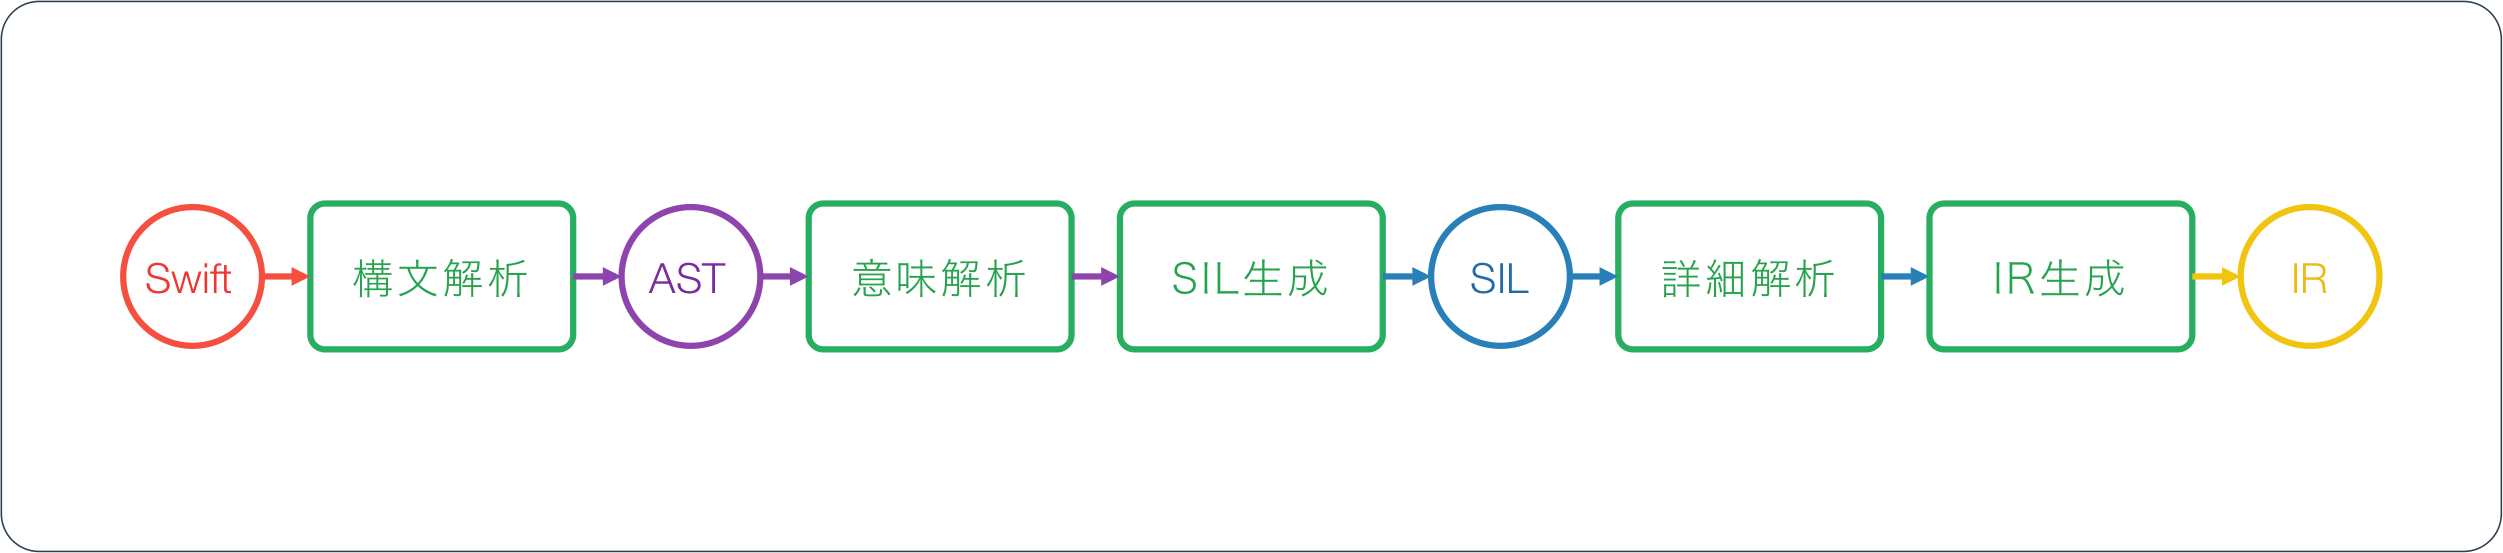
\includegraphics[scale=0.30]{./img/swift_compile_process}
%         \caption{Swiftコンパイラの構成}
%         \label{img:swift-compile-process}
%     \end{center}
% \end{figure}
%
% 構文解析の詳細については~\ref{explain-swift:structure:parser}節で詳しく述べるが、Swiftコンパイラは構文解析時に可能な限り変数や型などの参照を解決し、続く意味解析で不明だった参照の解決と明示されていない型の推論、型の整合性の検査を行う。
%
% また、コンパイラの構成で特に特徴的なのは意味解析とLLVM-IRのコード生成との間にSIL(Swift Intermediate Language)という独自の中間表現を挟んでいる点である。
% Swiftコンパイラでは、このSIL形式でAST(Abstruct Syntax Tree)では解析しづらいコールグラフやクラス階層に基づくエラーの検出やメモリ管理用コードの挿入、最適化などを行っている。
%
% SIL形式が複雑な解析部分を担っているためにSwiftコンパイラの構文解析器とASTは意味解析より後のステップで更に改変されること無く、完全に分離されている。
% そのため、コンパイラ中の構文解析部分のみを抽出して他の実装と比較評価を行うことが可能となっている。
%
%
% \subsection{構文解析器の構成}
% \label{explain-swift:structure:parser}
%
% ~\ref{explain-swift:features}節で述べたようにSwiftは多くの特徴を持っているため、その構文は他の言語と比較しても複雑なものとなっており、構文解析には高い柔軟性が求められる。
% 以下ではSwiftコンパイラの構文解析器における各機能についてその特徴を述べる。
%
% \subsubsection{字句解析}
%
% \subsubsection{LL(k)方式構文解析}
%
% 現行のSwiftコンパイラでは再帰下降構文解析の一種であるLL(k)方式を構文解析に採用しており、その構文解析器はC++の関数として書き下されている。
%
% LL(k)方式では解析する対象の構文によって解析器が先読みを行うトークンの数を変更することで、各構文に必要な先読みの数を最小限に抑えながらも、~\ref{explain-swift:features:readability}節で取り上げたような完全な曖昧性を持つ構文以外は必ず解析対象の構文を決定することができる。
%
% また、単なるLL(k)方式の構文解析器が自動生成が可能であることは~\cite{antlr}などで知られているが、Swiftの場合は先述の曖昧な構文に対する対処やより詳細なエラーの報告を行うために、構文解析器を全て手動で書き下している。
%
% \subsubsection{参照解決}
%
% 現行のSwiftコンパイラでは構文解析時に可能な限り変数や型の参照を解決し、他のファイルで宣言されている可能性のあるものなど、その時点で解決不可能なものについては解決不可能としてマークしてASTに組み入れる。
% 解決が不可能であった参照は全てのファイルを走査し終えた後の意味解析の最初のステップで解決される。
%
% \subsubsection{スコープ解決}
%
% \subsubsection{AST}
%
% \subsubsection{曖昧な構文の解析}
%
% Swiftコンパイラの構文解析器では、構文定義的に参照の解決などが行われた後でなければどの構文なのかを判断することができない曖昧な構文については、ひとまず特定の構文として解析して意味解析時に適切な形式でなかった場合にのみそれを変換する。

%%% Local Variables:
%%% mode: japanese-latex
%%% TeX-master: "../thesis"
%%% End:
